\lab{Python}{Vectorization}{Vectorization}
\label{lab:Python_Vectorization}

In Python, the cost of looping over a sequence is sometimes prohibitive.
One method for avoiding these explicit for-loops is to \emph{vectorize} our code.
NumPy allows operation that normally apply only to scalars to also work seamlessly with NumPy arrays.
Some of the benefits of allowing these types of operations are concise code and fast execution.

\section*{Some Simple Examples}

Vectorization is a term that refers generally to the eliminating of for-loops in higher level languages as well as taking advantage of the capabilities of modern processors to perform the same operaiton on multiple numbers at once.
We'll start with a very simple example.
The following code takes the sum of the elements of a NumPy array.
\begin{lstlisting}
def pysum(A):
    total = 0.
    for i in xrange(A.size):
        total += A[i]
    return total
\end{lstlisting}
At each stage it accesses the array which involves the creation of a new Python object to contain the floating point value in that portion of the array.
This slows down the operations significantly.
We can avoid creating and deleting a Python object by doing the operations in a lower level language like C or FORTRAN.
NumPy has already implemented many of these basic operations for us in these lower level languages.
Many of these operations in NumPy also take advantage of multithreading, which allows for the processing of multiple array elements at once.
In this case, we can just use the \li{sum()} method of arrays.
Timing the results, we see a significant speedup.
\begin{lstlisting}
>>> import numpy as np
>>> from numpy.random import rand
>>> A = rand(1000000)
>>> %timeit pysum(A)
1 loops, best of 3: 3.25 s per loop
>>> %timeit A.sum()
100 loops, best of 3: 12.9 ms per loop
\end{lstlisting}
This is a remarkable speedup.
Even for such a simple operation we see a speedup of a factor of 250!

We now consider an example of an operation that is not built in to NumPy.
Consider a two dimensional array where each row represents a point in $\mathbb{R}^n$.
To make computation nice, lets say that the norm of each point is neither extremely large nor extremely small.
The following code normalizes the vectors represented in the array by modifying it in place:
\begin{lstlisting}
from math import sqrt
def normalize1(A):
    # for each row (point) in A
    for i in xrange(A.shape[0]):
        # Compute norm
        # Start by summing
        # squares of entries in this row.
        total = 0.
        for j in xrange(A.shape[1]):
            total += A[i,j]**2
        # take square root to get norm
        total = sqrt(total)
        # divide row by its norm
        for j in xrange(A.shape[1]):
            A[i,j] /= total
\end{lstlisting}
This problem can be vectorized in stages.
Here we will proceed by eliminating the inner for-loops, then eliminate the outer one.
The inner for-loops can be eliminated like this:
\begin{lstlisting}
def normalize2(A):
    # for each row (point) in A
    for i in xrange(A.shape[0]):
        # compute norm of row
        # then divide it by its norm
        A[i] /= sqrt((A[i]**2).sum())
\end{lstlisting}
This is much shorter, much faster, and reads quite nicely.
It is also usually faster than the original.
To eliminate the last for-loop we do the computation for all the rows at once.
\begin{lstlisting}
def normalize3(A):
    # compute the norm of each row
    # then divide each row by its norm
    A /= np.sqrt((A**2).sum(axis=1,keepdims=True))
\end{lstlisting}
At a glance, what this line does may be a little less clear.
It essentially takes the square of \li{A}, sums its columns (i.e. sums along its rows), takes the square root, then divides \li{A} by the result by broadcasting along rows.
The \li{keepdims} option is used to align the axes for broadcasting.
An equivalent line of code would be \li{A /= np.sqrt((A**2).sum(axis=1).reshape((A.shape[0],1)))}.
Timing our results we see that eliminating these loops and allowing NumPy to perform some of these operations in parallel results in a significant speedup.
\begin{lstlisting}
>>> A = rand(1000000, 2) # 10^6 2D points
>>> Ac = A.copy()
>>> %time normalize1(A)
Wall time: 8.6 s
>>> A[:] = Ac
>>> %time normalize2(A)
Wall time: 14.3 s
>>> A[:] = Ac
>>> %time normalize3(A)
Wall time: 68 ms
>>> A = rand(1000000, 20) # 10^6 20D points
>>> Ac = A.copy()
>>> %time normalize1(A)
Wall time: 58.5 s
>>> A[:] = Ac
>>> %time normalize2(A)
Wall time: 14.6 s
>>> A[:] = Ac
>>> %time normalize3(A)
Wall time: 250 ms
>>> A = rand(50, 10000000) # 50 (10^7)D points
>>> Ac = A.copy()
>>> %time normalize2(A)
Wall time: 5.38 s
>>> A[:] = Ac
>>> %time normalize3(A)
Wall time: 5.4 s
\end{lstlisting}
Notice how much the dimensions of \li{A} affect the performance of each algorithm.
The first one is slowed down by its extensive use of Python objects for basic computations.
The second one is slowed down by the fact that it makes a new array slice for each row.
The third is slowed down by the fact that it must allocate a significant amount of temporary storage in memory to perform all its computations.
A faster and more memory-efficient solution to this problem can be obtained, but it required using another language (like C, C++, Cython, or FORTRAN) that better optimizes for-loops.
As always, when optimizing keep in mind that it takes extra time to optimize code.
A partial optimization is often good enough.
In general, only optimize when you are sure it will be worth your time to do so.

\section*{Vectorization Techniques}

Here are a few specific techniqes that can be useful in vectorization.

\begin{itemize}

\item Try to manipulate your computations mathematically.
Changing the order or way operations are applied can (but does not always) improve speed significantly.
A very simple example is $\sin^2 x + \cos^2 x = 1$.
Another example is that, for an orthogonal matrix, $A^{-1} = A^T$.
A transpose is a constant time operation because all that is required is creating a new view of the same memory.
A matrix inversion is much more expensive.

\item Try to avoid allocating unnecessary temporary arrays.
Long algebraic expressions in NumPy often involve the creation of large amounts of temporary arrays.
Excessive memory use limits the size of the problems your code can handle and slows it down.
This will be discussed further in a later lab, but be careful.

\item Eliminate the longer for-loops in Python.
Python's loops are much slower than the loops that are run in other languages like C and FORTRAN.
Many simple loops involving basic numeric operations can be performed in these languages through NumPy's built in functions.
This is an easy place to start optimizing.

\item Watch for times when broadcasting might be convenient.
This will save memory and let your program avoid unnecessary computations.

\item Use NumPy's universal functions.
It is much faster to evaluate something like \li{np.sin(x)} than something like
\begin{lstlisting}
from math import sin
Asin = np.empty_like(A)
for i in xrange(A.size):
    Asin[i] = sin(A[i])
\end{lstlisting}

\item In general, use common sense.
Think about the operations required to perform each computation.
Try out different implementations and compare their strengths and weaknesses, then use your best judgement about what the most common uses will be.
When optimizing, make absolutely sure to test your code to verify that you are getting the expected results.
Also be sure to comment your code carefully so that you (or whoever has to read your code) will be able to tell what you are doing.
Often it is more important to make code readable than it is to make it fast.
Use your best judgment.

\end{itemize}

To demonstrate the above principles we'll consider another example.
We will write a function which, given two arrays \li{A} and \li{B} will return the distance from \emph{each} point of \li{A} to \emph{every} point of \li{B}.
This can be done naively using for-loops as follows:
\begin{lstlisting}
from math import sqrt
import numpy as np
def dist1(A, B):
    # Preallocate output array.
    # Start with everything set to 0.
    D = np.zeros((A.shape[0], B.shape[0]))
    # For each row in A
    for i in xrange(A.shape[0]):
        # For each row in B
        for j in xrange(B.shape[0]):
            # For corresponding entries of
            # the rows in A and B
            for k in xrange(A.shape[1]):
                # add the squared difference
                D[i,j] += (A[i,k] - B[j,k])**2
            # take square root after finishing sum
            D[i,j] = sqrt(D[i,j])
    return D
\end{lstlisting}
We can eliminate the innermost for-loop easily
\begin{lstlisting}
def dist2(A, B):
    # Preallocate output array.
    # This time we'll be overwriting it,
    # so there's no need to assign it values.
    D = np.empty((A.shape[0], B.shape[0]))
    # For each row in A
    for i in xrange(A.shape[0]):
        # For each row in B
        for j in xrange(B.shape[0]):
            # Take the distance between the rows
            D[i,j] = sqrt(((A[i] - B[j])**2).sum())
    return D
\end{lstlisting}
Using the \li{axis} argument of the \li{sum()} method of arrays we can eliminate the next for-loop like this:
\begin{lstlisting}
def dist3(A, B):
    # Preallocate output array
    D = np.empty((A.shape[0], B.shape[0]))
    # For each row in A
    for i in xrange(A.shape[0]):
        # Take distance from this row to each row in B.
        # Use np.sqrt to operate on the entire array at once.
        D[i] = np.sqrt(((A[i] - B)**2).sum(axis=1))
    return D
\end{lstlisting}
This is a fairly nice solution.
It can be improved further.
Our final solution will take advantage of the fact that $\left(a - b\right)^2 = a^2 + b^2 - 2 a b$.
It will also use array broadcasting and in place operations to avoid excess memory use.
For many applications the above solution is good enough, but that isn't always the case.
\begin{lstlisting}
def dist4(A, B):
    # Use the fact that
    # (a-b)**2 = a**2 + b**2 - 2*a*b
    # Take squares of A and B.
    # Reshape so broadcasting works later
    A2 = (A**2).sum(axis=1).reshape((-1,1))
    B2 = (B**2).sum(axis=1).reshape((1,-1))
    # Use matrix multiplication to start
    # computing the remaining term.
    D = A.dot(B.T)
    # Multiply in place to avoid
    # allocating temporary arrays.
    # Notice that this operates on
    # the entire array.
    D *= -2
    # Broadcast to add in A2 and B2.
    # Perform these operations in place.
    D += A2
    D += B2
    # Take square root without
    # allocating a temporary array.
    np.sqrt(D, out=D)
    return D
\end{lstlisting}
Depending on how you are using your squared distance you could also use the fact that for $x, y \geq 0$, $x < y$ if and only if $\sqrt{x} < \sqrt{y}$.
This would be useful if all you need to know is which distances are greater than one another.
Timing these functions gives the following results:
\begin{lstlisting}
>>> A = rand(500, 2)
>>> B = rand(1000, 2)
>>> %timeit dist1(A, B)
1 loops, best of 3: 3.18 s per loop
>>> %timeit dist2(A, B)
1 loops, best of 3: 6.86 s per loop
>>> %timeit dist3(A, B)
10 loops, best of 3: 27.6 ms per loop
>>> %timeit dist4(A, B)
100 loops, best of 3: 7.51 ms per loop
>>> A = rand(500, 20)
>>> B = rand(1000, 20)
>>> %timeit dist1(A, B)
1 loops, best of 3: 23.8 s per loop
>>> %timeit dist2(A, B)
1 loops, best of 3: 6.89 s per loop
>>> %timeit dist3(A, B)
10 loops, best of 3: 60.5 ms per loop
>>> %timeit dist4(A, B)
100 loops, best of 3: 7.82 ms per loop
>>> A = rand(50, 200)
>>> B = rand(100, 200)
>>> %timeit dist1(A, B)
1 loops, best of 3: 2.29 s per loop
>>> %timeit dist2(A, B)
10 loops, best of 3: 71.9 ms per loop
>>> %timeit dist3(A, B)
100 loops, best of 3: 5.28 ms per loop
>>> %timeit dist4(A, B)
1000 loops, best of 3: 283 µs per loop
\end{lstlisting}
As you can see, the dimensions of the problem still change how long it will take.
In every case the final solution was the fastest.
Proper vectorization has, in this case, given a speedup by more than a factor of 1000 while still using a fairly reasonable amount of memory.
Plots of the times for these different functions can be seen in Figure \ref{distplot}.

\begin{figure}
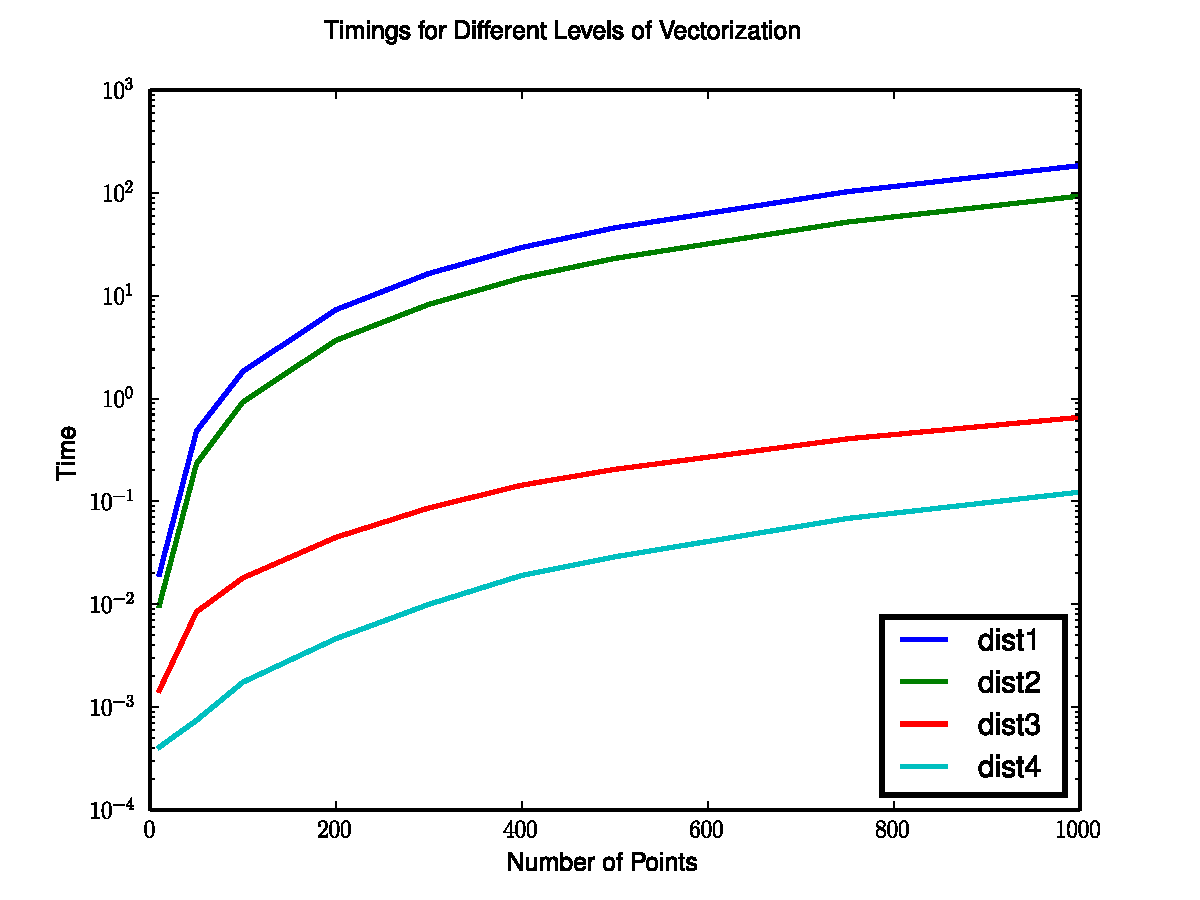
\includegraphics[width=\textwidth]{distplot.pdf}
\caption{A plot of the times for the different degrees of vectorization for a function finding the distance between points represented as rows in two arrays. Arrays of points in $\mathbb{R}^{10}$ were used for this computation.}
\label{distplot}
\end{figure}

\begin{problem}
Use vectorization techniques to obtain an optimized solution to each of the following problems.
They can all be done in one line.

\begin{enumerate}[a)]

\item For an array \li{X} compute the inner product of each row with each other row.
Hint: Think matrix multiplication.

\item For an array of points \li{X} where each row represents a point in $\mathbb{R}^n$ compute $\| x\|^2$ for each row \li{x} of \li{X}.
Hint: Use array multiplication instead of matrix multiplication for this one.

\item Compute the matrix expression $v^T A v$ where $A$ is a square matrix and each column vector $v$ is stored as a row in an array \li{V}.
The shapes of \li{V} and \li{A} are \li{(n, d)} and \li{(n, n)} respectively.
Hint: Matrix multiplication, then array multiplicaiton, then a sum along an axis.

\item For an array \li{A} of size \li{n} count the number of elements of \li{A} less than $\frac{1}{2}$.
Hint: Sum over a boolean array.

\item Modify an array \li{A} of size \li{n} and set every value less than $\frac{1}{4}$ to $0$.
Hint: Use fancy indexing.

\item Given an array \li{A} of shape \li{(n, n)} representing a linear transform on $\mathbb{R}^n$, apply \li{A} to an array of points \li{X} where each row of \li{X} is a point in $\mathbb{R}^n$.
Hint: This is all about transposes and matrix multiplication

\item For an array \li{A} of shape \li{(m, n, n)} which represents $m$ linear transformations from $\mathbb{R}^n$ to $\mathbb{R}^n$ and an array \li{X} of shape \li{(k, n)} whose rows represent points in $\mathbb{R}^n$ compute the image of each row of \li{X} under each transformation represented in \li{A}.
Format the results so the have shape \li{(m, k, n)}.
Hint: Do a matrix multiplication, then use the \li{swapaxes()} method of an array to rearrange the axes properly.

\item Let \li{A} be an array of shape \li{(m, n)} and \li{B} be an array of shape \li{m}.
Take the sum of every element of \li{A} that lies in a row of \li{A} with a first element that is less than $\frac{1}{2}$.
Hint: Use matrix multiplication by a row vector of boolean values.

\item For an array \li{P} of shape \li{n} and a boolean array of shape \li{D} compute the array \li{A} such that \li{A[i]} is $\sum_{D[i,j] = True} \left( P[i] - P[j]\right)$.
Hint: For each \li{i} let $k_i = \sum_{D[i,j] = True} 1$ (the number of \li{True} values , then the \li{i}'th entry of \li{A} should be $k_i * P[i] - \sum_{D[i,j] = True} P[j]$.
The first part of this expression can be evaluated by array multiplication and a sum across an axis.
The second part can be evaluated with matrix multiplication.

\item Shuffle a one-dimensional array of values the way you would shuffle a deck of cards, i.e. separate it into two stacks, then take every other item from each of the two stacks.
Hint: This can be done with array slicing and multiple assignment (i.e. \li{a, b = c, d}).
To make the assignment work nicely with the slicing, be sure to use copies of both slices.
Note: In general this isn't how you would do this.
A purely random arrangement of rows can be obtained using \li{numpy.random.shuffle()}.

\end{enumerate}
\end{problem}

\section*{Image Editor}
An image is often represented as a 3D array where the first and second dimensions are the height and width respectively and the third dimension represents the intensity of each of three color channels: red, green, and blue.
The code below can be used to read and display images in Python.
\begin{lstlisting}
import matplotlib.pyplot as plt
img = plt.imread(<image-file>)
plt.imshow(img)
plt.show()
\end{lstlisting}

Matplotlib can read in PNG images on its own, otherwise it will read in images using the Python Image Library.
Depending on the format of the image, it may be read as an array of floating point values between 0 and 1 or it may be read as an array of integer values between 0 and 255.
In this lab we will assume the latter.

\begin{problem}
Use vectorization techniques to obtain an optimized solution to each of the following problems.
They can all be done in one line.
\begin{enumerate}[a)]

\item Given an array representing a color image, make an array representing a black and white image where the black and white value is the average of each of the color values.
Hint: see the \li{mean()} method of arrays.

\item For an array representing a color image calculate the absolute value of the difference between each color value and the average value for each pixel.
Hint: pass the \li{keepdims=True} argument to the \li{mean} method so tha broadcasting works properly.

\end{enumerate}
\end{problem}

\begin{problem}
Write a function that edits an array representing an image.
Include options that allow you to  invert the image, change it to grayscale, or add a motion blur (definitions below).
The function should take in an image, a parameter that indicates how to modify the image, and an optional parameter for the motion blur.
It should then plot the image.
\end{problem}

\begin{itemize}
\item Invert:
Every color value for every pixel is changed to its inverse value. For example, 0 becomes 255, 230 becomes 25, and 127 becomes 128.
Remember that the minimum color value is 0 and the maximum is 255.

\vfill
\begin{figure}[ht]
\begin{minipage}[b]{0.47\linewidth}
\centering

\includegraphics[width=\textwidth]{Original.png}
\end{minipage}
\hspace{0.1cm}
\begin{minipage}[b]{0.47\linewidth}
\centering

\includegraphics[width=\textwidth]{Invert.png}
\end{minipage}
\caption{Example of an inverted image}
\end{figure}
\vfill

\item Grayscale:
To convert an image to grayscale, each pixel's color value is changed to the average of
the pixel's red, green, and blue value. For example, if the pixel values are
Red: 225, Green:, 30 Blue: 131, we set each of these values to $\frac{225 + 30 + 131}{3} = 128$ (using integer division).
Hint: use the \li{axis} argument to the mean method of NumPy arrays.
To get integer division, use its \li{dtype} argument.

\vfill
\begin{figure}[ht]
\begin{minipage}[b]{0.47\linewidth}
\centering

\includegraphics[width=\textwidth]{Original.png}
\end{minipage}
\hspace{0.1cm}
\begin{minipage}[b]{0.47\linewidth}
\centering

\includegraphics[width=\textwidth]{Gray.png}
\end{minipage}
\caption{Example of an image that is grayscaled}
\end{figure}
\vfill

\item Motion Blur:
An additional parameter $n>0$ will be used for motion blur.
The value of each color of each pixel is the average of that color value for $n$ pixels (from
the current pixel to $n-1$ beyond) horizontally. So pixel \li{[x,y,0]} would turn in to the average of
pixel \li{[x,y,0]} to pixel \li{[x,y+n-1,0]}.
Note: You will need to use one for-loop here.
Be sure to account for the situations where one or more of the values used in the computing the average do not exist. For example, if an image has width $w$ and we are considering the pixel on row $r$, column $c$, if $c + n \ge w$, then we only average the pixels up to $w$. (Proper array slicing should take care of this case without any extra code.)

\vfill
\begin{figure}[ht]
\begin{minipage}[b]{0.47\linewidth}
\centering

\includegraphics[width=\textwidth]{Original.png}
\end{minipage}
\hspace{0.1cm}
\begin{minipage}[b]{0.47\linewidth}
\centering

\includegraphics[width=\textwidth]{Motion.png}
\end{minipage}
\caption{Example of an image with a motion blur of 60}
\end{figure}
\vfill

\end{itemize}

